\chapter{Evaluation}
\label{chap_eval}

\section{Protocol}

All experiments were conducted on the BU-3DFE database. The database contains $2,500$ scans of faces. There are $100$
persons ($44$ men and $56$ women) and each person performs $25$ expressions.
There is one neutral expression and every person expressed each of the $6$ emotions (anger, sadness,
happiness, surprise, disgust, fear) at $4$ intensity levels. The database is annotated, there are landmarks
with clear semantic meaning (like tip of the nose, eye corners, etc).
For training we need registered scans and we used the registration 
from \cite{Salazar}. It was performed with template fitting method
and some obvious mistakes were manually corrected by T. Bolkart.
The registered scans contain $5,996$ points each, so the mode-$1$ dimension
of the  uncompressed tensors is $17,988$.

We used the {$10$-fold} cross validation. 
The database was split into $10$ parts, each part containing the same number of males and females, and
each part was used as a testing dataset for models trained on the other $9$ parts, then the results
were averaged.


\section{Implementation details}


The implementation of Newton-Grassmann method
by Elden and Savas is available as part of Tensor Toolbox \cite{tensor_toolbox}.
The implementation of Differential-Geometric Newton method
is available as part of TensorLab package \cite{tensor_lab}.
Both these packages are written in Matlab and contain
also implementations of HOOI and HOSVD, too.

Nevertheless, it was necessary to re-implement the methods
for two reasons.
First, we solve the Tucker2 decomposition problem, not the
full decomposition.  The unfolding $X_{(1)}$ in our experiments
has the size $17,988 \times 2,250$ and has at most $2,250$ 
non-zero singular values. This means that even if we tried
to perform HOSVD without truncation in the first mode ($r_1 = d_1 = 17,988$),
it will fail.
The second, and more important reason is that the implementation
provided by the authors is usually aimed at working
with relatively small tensors. In the intermediate calculations
it is necessary to compute the matrices whose
dimension for our data would be too big to fit into memory.
We overcome this issue by computing the matrix of the 
system column-wise. Ishteva et al.
use GMRES solver in \cite{IDLAVH09} to solve the system \ref{?} without
explicit computation of the matrix. This approach could
be adapted in our case, but it may be interesting
to look at the condition numbers of system matrices, 
so we decided to compute them explicitly.
Third, if some of this methods proved to be much more
efficient than HOSVD, it would be necessary to integrate 
them into existing framework written in C++, anyway.





HOOI and Newton-Grassmann methods were implemented in C++ using the existing framework 
of Bolkart and Wuhrer (\cite{bolkart_wuhrer_2013}), that already had HOSVD implementation.
The implementation was done with Armadillo library (\cite{armadillo_report}),
which provides a Matlab-like wrapper for LAPACK.
The differential-geometric Newton method was implemented in Matlab,
where we used routines from  the tensor toolbox \cite{tensor_toolbox}.
The code for fitting was provided as part of the framework. The code for 
expression recognition was taken from Daniel Mohr's thesis
(it had to be changed to work with full scans instead of their subset
that corresponds to Kinect landmarks).




\subsection{HOSVD}
This method is very easy to implement and it is not iterative,
so the only parameters involved are truncated dimensions $r_2$
and $r_3$. The analysis performed in Bolkart and Wuhrer \cite{bolkart_wuhrer_2013}
showed that $r_2 = 30$ and $r_3 = 7$ is a reasonable choice of parameters (it gave 89 \% compactness
in the expression space and $90$ \% compactness in the identity space for the whole database,
our training datasets have almost the same size). Of course, the same dimensions
were used in all other methods.

\subsection{HOOI}

The method is also quite easy to implement. As for termination criterion,
we used the relative norm of the gradient with threshold $10^{-5}$. This threshold
is always achieved after $30$ iterations.



\subsection{Newton-Grassmann method}

Implementation of this method involves more work. We used initialization from HOOI after $4$ iterations (the relative
norm of the gradient is about $0.5$). If we implement the algorithm
using the fixed step size $1$, as in the paper \cite{elden_savas_2009},
then the algorithm is diverging and gives no improvement. This behaviour
does not change if we initialize the algorithm with the result of HOOI
after $30$ iterations. 
Since there is a general recommendation to use some optimization
for step size at each iteration in Newton's methods (\cite{num_recipes}),
we perform a simple binary search for step size
and stop iterations, if the step size is too small.
We must admit that, even though some small improvement
in terms of the residual can be achieved using this modification,
it still looks that the method is diverging.


We also computed eigenvalues and condition number of the system matrix,
that is, of the Hessian. The condition number was above $10^{20}$ for initialization
with $4$ HOOI iterations and approximately $10^4$ for initialization with $30$
HOOI iterations. If the Hessian was a definite matrix,
we could conclude that in this case we need to perform more
initialization steps to get closer to the extremum point.
However, in both cases the Hessian had both positive and negative
eigenvalues. The authors suggested the following heuristic technique: if the Hessian is not definite, we can diagonalize it, make all
eigenvalues in the diagonal matrix have the same sign and then solve the system with this tweaked Hessian matrix. However,
with our data this heuristic did not work.

\subsection{Differential-Geometric Newton method}
This method was implemented in Matlab.
In our implementation of the differential-geometric Newton method we
do not use an iterative solver, but explicitly compute the system
matrix. Even though
the final system matrix has a relatively small size ($2,875 \times 2,875$ in our
experiments), the intermediate calculations cannot be performed
in one step using vectorization rules,
due to the presence of several Kronecker product operations. 
Vectorization of this operation requires computation of very large (but sparse) matrices
whose size exceed the limits of Matlab. Therefore we computed the matrix of the system \eqref{dg_newt_system}
column by column (if $A$ is a matrix of a linear operator $\R^N \to \R^N$, then
the $i$th column of $A$ is the value of $A$ on the $i$th element of the standard
basis, $A(e_i)$). Clearly, this increases the running time by the factor of
order $3$, so the results for the running time of this algorithm in Table \ref{}
are given only for the sake of completeness.


This method also diverged when we initialized it with HOOI
performing either $4$ or $30$ iterations. We should mention
that there is no theoretical proof that the method
will converge to orthogonal matrices $F_2$, $F_3$, 
Ishteva et al. only make an empirical observation
that this was true in their experiments with tensors of the size $20 \times 20 \times 20$.
We modified the method by applying Gram-Schmidt orthogonalization process
after each step and performing
the same procedure for finding the optimal step size
as in Newton-Grassmann method. After this modification
the first $3$ or $4$ iterations
gave some very small improvement of the residual, but still diverged
for further iterations.


The condition number of the system matrix was always above $10^{20}$.

\section{Running time}

In most applications of the multilinear model the compression
is performed once, and the running time of the algorithm
is not too important. Nevertheless, it is possible to apply Minimum
Description Length principle to improve the correspondence between different
scans. In order to do this it is necessary to learn the model
at each iteration of the registration process, and the running
time is crucial here.


The theoretical time complexity estimates for the algorithms
is summarized in Ishteva \cite{ishteva_thesis}. If we compress in mode $k$
from $d$ dimensions to $r$ dimensions, then HOOI takes $O(d^3r + dr^4 + r^6)$,
and both Newton methods take $O(d^3 r^3)$.

The actual running time (averaged) is given in Table \ref{running_time_per_iteration}.
We see that Newton-Grassmann method takes significantly more time than HOOI.
As for differential-geometric Newton method, we have already mentioned
that our implementation is highly ineffecient, so the time given in the table
is not representative.

\begin{table}[h]
\centering
\begin{tabular}{|c|l|l|l|l|}
\hline
Method & HOSVD & HOOI & NG & DGN(*) \\ \hline
Running time/iteration, sec & $30$  & $35$  & $120$ & $3,600$ \\ \hline
\end{tabular}
\caption{Running time of different methods. NG stands for Newton-Grassmann
method, DGN stands for Differential-Geometric Newton method.}
\label{running_time_per_iteration}
\end{table}

\section{Frobenius norm}

The simplest measure of comparing different methods
is calculating the Frobenius norm of the residual $\| X - M \times_2 F_2 \times_3 F_3 \|$.
The average values of Frobenius norm are given in {Table \ref{frob-norm-residual}}:





\begin{table}[h]
\centering
\begin{tabular}{|c|c|c|}
\hline
Method                         & Average norm of the residual & Standard deviation \\ \hline
HOSVD                         & $11,756.3$   &  $157.59$      \\ \hline
HOOI-4                        & $11,475.02$  &  $158.78$     \\ \hline
HOOI-30                       & $11,475.0$   &  $158.76$     \\ \hline
NG              & $11,475.0$   &  $158.79$     \\ \hline
DGN &  $11,475.0$  &  $158.79$      \\ \hline
\end{tabular}
\caption{Values of the average Frobenius norm of the residual. HOOI-4 stands for $4$ iterations of HOOI; HOOI-30 stands for $30$ iterations of HOOI; NG stands for Newton-Grassmann method, DGN stands for Differential-Geometric Newton Method.}
\label{frob-norm-residual}
\end{table}


We see that HOOI gives some improvement in comparison to HOSVD,
while the effect of Newton methods is hardly noticeable (see remarks below). Note that it is the result of the
first $4$ iterations. In Figure \ref{fig:hooiimprove} we provide a typical dynamics of improvement of the norm of the residual for HOOI. 
Iteration $0$ corresponds to HOSVD. The effect of the first  iteration
of HOOI seems to be the most important, and it may look as if
improvement stops here. However, this is not true. We provide Figure \ref{fig:hooiimprove1}, a zoomed-in version of the previous plot, in which
we can clearly see that some significant improvement also happens 
in the first $4$ iterations.

\begin{figure}[ht!]
\centering
        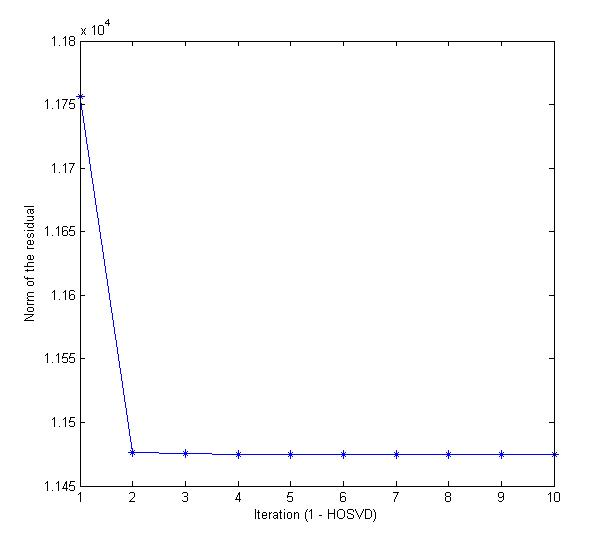
\includegraphics[height=2.3in]{images/hooi_hosvd_residual_plot}
        \caption{Improvement of the norm of the residual, with HOSVD}
    \label{fig:hooiimprove}
\end{figure}


\begin{figure}[ht!]
\centering
        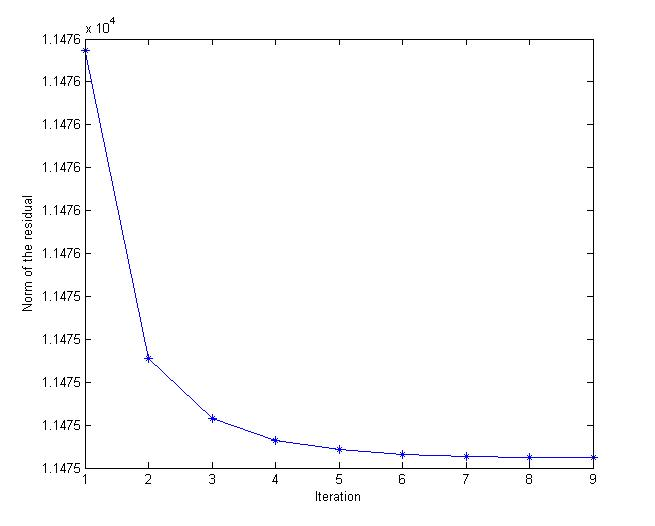
\includegraphics[height=2.3in]{images/hooi_residual_plot}
        \caption{Improvement of the norm of the residual, without HOSVD}
    \label{fig:hooiimprove1}
\end{figure}


The Figure \ref{fig:hooi_grad_plot} shows the dynamics of the
projected gradient. Note that the plot is in logarithmic scale.
We can see that, even though the norm of the residual practically
stopped changing after first $10$ iterations,
the norm of the gradient is decreasing quite fast even at iterations
$30$ to $40$. We conclude that for our data HOOI converges to 
a critical point.

\begin{figure}
        \centering
                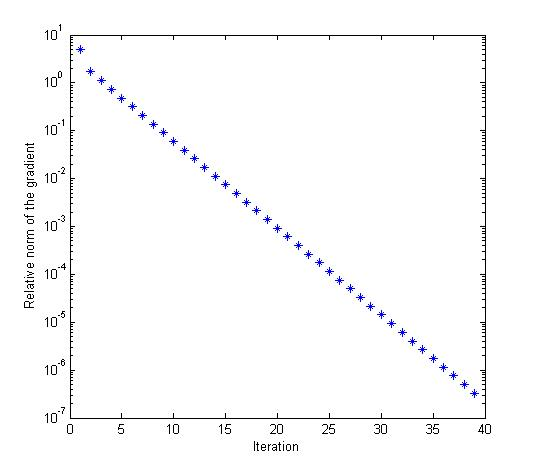
\includegraphics[width=8cm]{images/hooi_gradient_plot.jpg}
        \caption{Relative norm of the gradient (logarithmic scale).}
        \label{fig:hooi_grad_plot}
\end{figure}


As for Newton methods, they demonstrate some very small improvement
during first $4$ or $5$ iterations and then they started
diverging very fast. A typical example (for differential-geometric Newton method) is in Figure \ref{fig:grad_newgr}.
Note that the plot is in logarithmic scale. Due to the non-monotonicity of both Newton methods, in practice we observed
$4$ iterations more to be absolutely sure that this rapid increase is indeed a sign of divergence. 


\begin{figure}
        \centering
                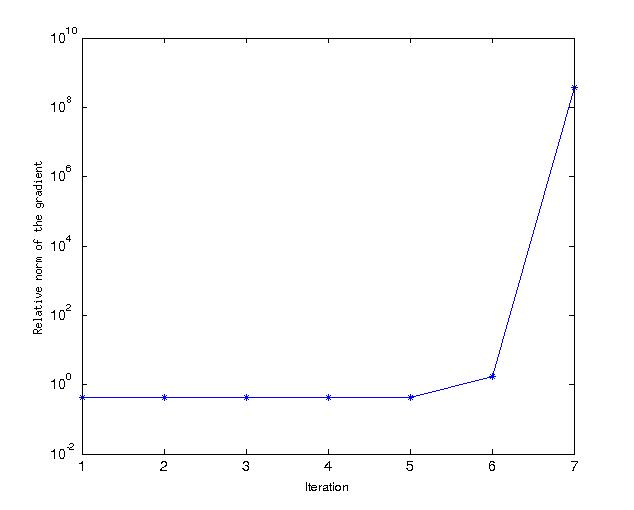
\includegraphics[width=8cm]{images/grad_newgr.jpg}
        \caption{Relative norm of the gradient in Differential-Geometric Newton method (logarithmic scale).}
        \label{fig:grad_newgr}
\end{figure}


\section{Reconstruction and Fitting}
\label{eval_fit}

The more application-relevant measure is fitting error: we take a face scan $\tilde{\f}$
from the testing dataset and try to fit it to the model. Recall the formulation of this from Section \ref{mult_model}.

\begin{equation}
\mbox{Find $\w_2 \in \R^{r_2}$, $\w_3 \in \R^{r_3}$ that minimize } \rho(\tilde{\f}, \f(\w_2, \w_3)) \to \min.
\end{equation}

Here $\f(\w_2, \w_3)$ denotes the reconstructed face $\bmu + \G \times_2 \w_2 \times_3 \w_3$. The fitting error
$\rho$ is defined to be
\begin{equation}
\rho(\tilde{\f}, \f) := \sum_{ p \in \f } dist(p, NN(p, \tilde{\f}),
\end{equation}
where $NN(p, \tf)$ is the nearest neighbour of point $p$ on the scan $\tf$. 


The actual procedure of fitting starts with finding a rigid transformation
that aligns the input scan with the mean face $\bmu$. After alignment
at each iteration the non-linear optimization procedure \textrm{vnl\_lbgfs} from the VNL library
is used to improve the weights.



If the input to the fitting procedure is a registered scan, not a scan from the original
database, then we call this procedure reconstruction. In this case
we wish the model to reproduce the face with the same correspondence. The reconstruction
error is measured by simply computing the distance between the points with the same
index in $\f$ and $\tf$. The reconstruction error is typically higher than the 
fitting error, since it is harder to satisfy the dense correspondence constraint.


The average values of the fitting and reconstruction errors are given in Table \ref{avg_fit_rec_error}.
We can see that there is no significant difference. Interestingly, HOSVD demonstrates
the worst results for fitting and the best results for reconstruction. However,
even though the difference between values of HOSVD and all other methods is more than the difference
between any other two methods, still it is too small to draw any conclusions.



The average values alone do not provide much information. It might be that for some methods
the distribution of errors is significantly different or that some methods perform much better
in certain regions of a face than other methods do. In order to be sure that this is not the case
we produced cumulative error plots and visualized average error per vertex using false colored models.
In Figure \ref{fig:cum_err_reconstruct}
we give the cumulative error plot for reconstruction with Newton-Grassmann method, in Figure \ref{fig:cum_err_fit}
we give the cumulative error plot for fitting with HOOI with $4$ iterations. Of course, the shapes of the curves are quite different, this again demonstrates that reconstruction with correspondence is significantly harder.
However, if we compare two different methods on the same problem, we shall hardly be able to see the difference, 
that is why we give just these two plots and not all $10$ of them.


\begin{table}[h]
\centering
\begin{tabular}{|c|c|c|}
\hline
Method                         & Average reconstruction error, mm & Average fitting error, mm \\ \hline
HOSVD                         & $3.3551 $   &  $ 1.3201 $      \\ \hline
HOOI-4                        & $3.3708$  &  $ 1.3184 $     \\ \hline
HOOI-30                       & $3.37410$   &  $ 1.3179 $     \\ \hline
NG                           & $ 3.3702 $   &  $ 1.3182  $   \\ \hline
DGN                          &  $3.3702 $  &  $ 1.3182 $      \\ \hline
\end{tabular}
\caption{Values of the average reconstruction and fitting errors. HOOI-4 stands for $4$ iterations of HOOI; HOOI-30 stands for $30$ iterations of HOOI; NG stands for Newton-Grassmann method, DGN stands for Differential-Geometric Newton Method.}
\label{avg_fit_rec_error}
\end{table}


\begin{figure}
        \centering
                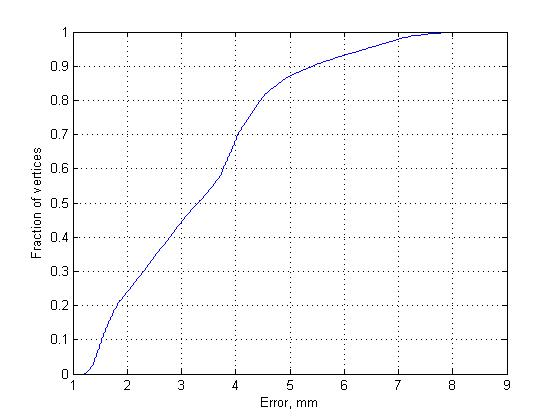
\includegraphics[width=8cm]{images/cum_error_rec_newgr.jpg}
        \caption{Cumulative error plot for reconstruction with Newton-Grassmann. For example, $70 $ \% of all vertices have error less than $4$ mm.}
        \label{fig:cum_err_fit}
\end{figure}

\begin{figure}
        \centering
                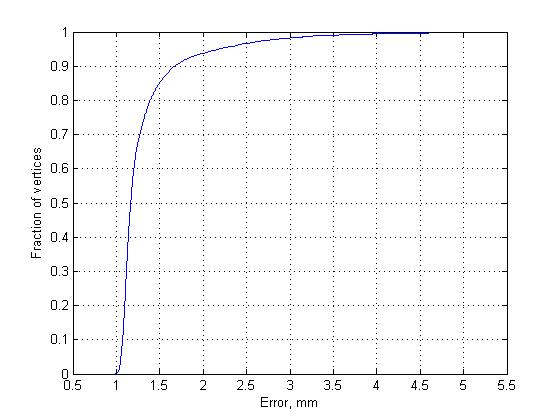
\includegraphics[width=8cm]{images/cum_error_fit_hooi_4.jpg}
        \caption{Cumulative error plot for fitting with HOOI. For example, about $84 $ \% of all vertices have error less than $1.5$ mm.}
        \label{fig:cum_err_fit}
\end{figure}




% In addition, we plot
%the average error per vertex in Figure \ref{avg_fit_rec_error}. The green areas correspond
%to the vertices where the average error is low, the red areas indicate vertices
%where the error is high. There is again no significant difference in the distribution
%of the error on face. 

\section{Expression Recognition}


We consider two approaches to the expression recognition problem.
The first step in both of them is
to fit the input scan $\tf$ to the model and get identity 
and expression weights.  

The most straightforward approach uses a simple nearest-neighbour classification.
We do not fit the scans of the training database to the model, but simply use
the columns of the projection matrix responsible for expression as representatives
of all faces in the training dataset that have this expression. This gives us $24$ (we ignore neutral
expression)
points in $\R^7$. We take the expression weight of the testing scan, search for
its nearest neighbour among these $24$ points and return the corresponding expression.
Maybe, it would be more accurate to actually fit the training scans
to the model and then we would have much more samples in the expression space.
However, fitting takes time and, more importantly, its 
results heavily depend on the initialization. If we choose
the corresponding column of the projection matrix
as an initial expression weight for fitting procedure (which 
seems to be a very reasonable choice), we should
get the final expression weight that is not too 
far way from this initial value.


The more involved approach was inspired by Mpiperis et al. \cite{mpip_2008}.
Before we start classification, we reconstruct the original faces using the learnt model.
Let $\G$ be the core tensor of the model, $F_2$ and $F_3$ be the projection matrices. The reconstructed
faces are (by definition) sums of the mean face $\bmu$ and mode-$1$ fibers of the tensor $\G \times_2 F_2^T \times_3 F_3^T$.

Now let $\f$ be an input scan from the testing dataset. The fitting procedure
gives us the identity and expression weights $\w_2$, $\w_3$. We can now reconstruct
the approximate version of $\f$ using the model as
\begin{equation}
\tf := \bmu + \G \times_2 \w_2^T \times_3 \w_3^T.
\end{equation}
Now each of the reconstructed faces of the training dataset casts a vote for its expression.
The vote is a real number proportional to $\exp( - d^2 / \sigma)$. Here $d$ is the
distance between the reconstructed face from the training dataset and $\tf$,
and $\sigma$ is some constant. All votes are summed up, and the expression
that obtained the maximal sum of votes is returned as the output
of the classification procedure.


In fact, we were slightly inaccurate when said that $d$ is the distance 
between $\tf$ and a reconstructed face from the training dataset. There are many
points that are not relevant for many expressions, and the noise from them,
when added up, may confuse the classifier. Instead of measuring distance
between all the corresponding points in both faces, only a subset is chosen
and the distances between corresponding points from that subset are added up
to make $d$.




\begin{table}[h]
\centering
\begin{tabular}{|l|l|l|l|l|l|l|}
\hline
Ground Truth\\Classified as    & Angry & Disgust & Fear & Happy & Sad & Surprised \\ \hline


Angry     &  	 54.50 	 &  11.00 	 &  8.25 	 &  2.25 	 &  23.00 	 &  1.00 \\ 
Disgust   &  	 29.25 	 &  44.00 	 &  12.00 	 &  3.75 	 &  6.75 	 &  4.25 \\ 
Fear      &  	 18.50 	 &  6.75 	 &  32.50 	 &  18.50 	 &  18.00 	 &  5.75 \\ 
Happy     &  	 23.00 	 &  4.75 	 &  23.25 	 &  38.75 	 &  6.00 	 &  4.25 \\
Sad       &  	 26.25 	 &  7.25 	 &  14.75 	 &  1.75 	 &  49.00 	 &  1.00 \\
Surprised &  	 25.25 	 &  2.25 	 &  6.50 	 &  4.50 	 &  27.75 	 &  33.75 \\ \hline

\end{tabular}
\caption{Confusion matrix for expression recognition, HOSVD }
\label{expr_rec_hosvd_confmatr_nn}
\end{table}


\begin{table}[h]
\centering
\begin{tabular}{|l|l|l|l|l|l|l|}
\hline
Ground Truth\\Classified as    & Angry & Disgust & Fear & Happy & Sad & Surprised \\ \hline

Angry     &  	 53.25 	 &  11.50 	 &  9.50 	 &  1.00 	 &  24.75 	 &  0.00 \\
Disgust   &  	 28.25 	 &  47.50 	 &  10.50 	 &  3.75 	 &  6.75 	 &  3.25 \\
Fear      &  	 20.75 	 &  8.50 	 &  33.25 	 &  13.75 	 &  16.50 	 &  7.25 \\
Happy     &  	 19.00 	 &  8.00 	 &  25.75 	 &  38.25 	 &  4.75 	 &  4.25 \\
Sad       &  	 21.25 	 &  7.50 	 &  14.25 	 &  2.00 	 &  54.25 	 &  0.75 \\
Surprised &  	 20.25 	 &  1.75 	 &  8.00 	 &  5.25 	 &  30.50 	 &  34.25 \\ \hline
\caption{Confusion matrix for expression recognition, HOOI, 4 iterations }
\label{expr_rec_hooi_confmatr_nn}
\end{table}


\begin{table}[h]
\centering
\begin{tabular}{|l|l|l|l|l|l|l|}
\hline
Ground Truth\\Classified as    & Angry & Disgust & Fear & Happy & Sad & Surprised \\ \hline
Angry     &  	 49.25 	 &  11.75 	 &  9.50 	 &  1.50 	 &  27.75 	 &  0.25 \\
Disgust   &  	 31.00 	 &  44.75 	 &  9.00 	 &  4.00 	 &  7.75 	 &  3.50 \\
Fear      &  	 20.00 	 &  8.25 	 &  32.75 	 &  14.50 	 &  18.00 	 &  6.50 \\
Happy     &  	 17.25 	 &  7.25 	 &  23.50 	 &  42.00 	 &  5.50 	 &  4.50 \\
Sad       &  	 23.50 	 &  7.25 	 &  11.75 	 &  1.75 	 &  54.00 	 &  1.75 \\
Surprised &  	 19.50 	 &  3.25 	 &  6.75 	 &  5.00 	 &  35.50 	 &  30.00 \\ \hline

\caption{Confusion matrix for expression recognition, HOOI, 30 iterations }
\label{expr_rec_hooi_30_confmatr_nn}
\end{table}


\begin{table}[h]
\centering
\begin{tabular}{|l|l|l|l|l|l|l|}
\hline
Ground Truth\\Classified as    & Angry & Disgust & Fear & Happy & Sad & Surprised \\ \hline
Angry     &  	 52.50 	 &  12.00 	 &  9.25 	 &  1.00 	 &  25.25 	 &  0.00 \\
Disgust   &  	 30.50 	 &  46.25 	 &  10.00 	 &  3.75 	 &  6.25 	 &  3.25 \\
Fear      &  	 20.00 	 &  7.50 	 &  34.50 	 &  14.25 	 &  16.75 	 &  7.00 \\
Happy     &  	 18.75 	 &  7.00 	 &  27.25 	 &  38.25 	 &  4.50 	 &  4.25 \\
Sad       &  	 21.75 	 &  7.75 	 &  13.25 	 &  2.00 	 &  54.50 	 &  0.75 \\
Surprised &  	 20.25 	 &  2.25 	 &  8.00 	 &  5.50 	 &  29.75 	 &  34.25 \\

\end{tabular}
\caption{Confusion matrix for expression recognition, Newton-Grassmann}
\label{expr_rec_newgr_confmatr_nn}
\end{table}


\begin{table}[h]
\centering
\begin{tabular}{|l|l|l|l|l|l|l|}
\hline
Ground Truth\\Classified as    & Angry & Disgust & Fear & Happy & Sad & Surprised \\ \hline
Angry     &  	 53.50 	 &  12.50 	 &  10.75 	 &  0.75 	 &  22.25 	 &  0.25 \\
Disgust   &  	 30.50 	 &  46.50 	 &  11.25 	 &  2.50 	 &  6.00 	 &  3.25 \\
Fear      &  	 20.75 	 &  9.00 	 &  32.25 	 &  15.00 	 &  16.75 	 &  6.25 \\
Happy     &  	 20.00 	 &  5.75 	 &  28.50 	 &  37.75 	 &  4.25 	 &  3.75 \\
Sad       &  	 22.75 	 &  8.25 	 &  13.50 	 &  2.00 	 &  52.75 	 &  0.75 \\
Surprised &  	 19.50 	 &  1.75 	 &  8.00 	 &  5.00 	 &  30.00 	 &  35.75 \\ \hline
\end{tabular}
\caption{Confusion matrix for expression recognition, Differential-Geometric Newton}
\label{expr_rec_dg_newton_confmatr_nn}
\end{table}

\begin{table}[h]
\centering
\begin{tabular}{|c|l|l|l|l|l|}
\hline
                            Method              & HOSVD & HOOI-4 & HOOI-30 & NG & DGN \\ \hline
Classification rate, NN, \%                         & $42.0833$  & $43.4583$ & $42.125$ & $ 43.375 $ & $43.0833$ \\ \hline
Classification rate, with reconstruction            & $ 40.25 $  & $39.75 $  & $ 37.7917$ & $ 39.7083$ & $39.875 $ \\ \hline
\end{tabular}
\caption{Expression recognition rate, comparison}
\label{expr_rec_rate_total}
\end{table}
